  
% Template for a Computer Science Tripos Part II project dissertation
\documentclass[12pt,a4paper,twoside,openright]{report}
\usepackage[pdfborder={0 0 0}]{hyperref}    % turns references into hyperlinks
\usepackage[margin=25mm]{geometry}  % adjusts page layout
\usepackage{graphicx}  % allows inclusion of PDF, PNG and JPG images
\usepackage{verbatim}
\usepackage{docmute}   % only needed to allow inclusion of proposal.tex
\usepackage[utf8]{inputenc}
\usepackage[T1]{fontenc}
\usepackage{tabularx}
\usepackage{ragged2e}
\newcolumntype{Y}{>{\RaggedRight\centering\arraybackslash}X}
\usepackage{booktabs}
\usepackage{changepage}
\usepackage{tikz}
\usepackage{tikz-3dplot}
\usepackage{eqnarray}
\usepackage{amsmath}
\usepackage{systeme}
\usepackage{cases}
\usepackage{amsthm}

% \usepackage{wrapfig}
\raggedbottom                           % try to avoid widows and orphans
\sloppy
\clubpenalty1000%
\widowpenalty1000%

\renewcommand{\baselinestretch}{1.1}    % adjust line spacing to make
                                        % more readable

\begin{document}

\bibliographystyle{plain}


%%%%%%%%%%%%%%%%%%%%%%%%%%%%%%%%%%%%%%%%%%%%%%%%%%%%%%%%%%%%%%%%%%%%%%%%
% Title

\pagestyle{empty}

%\rightline{\LARGE \textbf{}}

%\vspace*{30mm}
\begin{center}
\begin{Huge}
Part II Project\\
\textbf{Constructing 3D Models from Image Sequences} \\[5mm]
Ilinca Gabriela Sorescu \\
\end{Huge}
%\linebreak[5]
\vspace*{10mm}
\centerline{
\includegraphics[scale=0.2]{figs/Newnham_crest.png}}
\Large Newnham College \\
\vspace*{65mm}
\large \today % today's date
\end{center}

%%%%%%%%%%%%%%%%%%%%%%%%%%%%%%%%%%%%%%%%%%%%%%%%%%%%%%%%%%%%%%%%%%%%%%%%%%%%%%
% Proforma, table of contents and list of figures

\pagestyle{plain}

\chapter*{Proforma}

{\large
\begin{tabular}{ll}
Name:               & \bf Ilinca Gabriela Sorescu                       \\
College:            & \bf Newnham College                               \\
Project Title:      & \bf Constructing 3D Models from Image Sequences   \\
Examination:        & \bf Computer Science Tripos -- Part II, July 2015  \\
Word Count:         & \bf  \\
Project Originator: & I. G. Sorescu                     \\
Supervisor:         & Karina Palyutina                  \\ 
\end{tabular}
}



\section*{Original Aims of the Project}
The design and implementation of a system which emulates the shape of a 3D model by first producing a sequence of snapshots of the input model as seen from multiple viewpoints and then constructing a new model which resembles the original input from these snapshots. This system must be accompanied by an evaluation module which will test the accuracy of the outcome.


\section*{Work Completed}
All objectives drafted in the project proposal have been met: a system which generates snapshots of a 3D model has been assembled, along with a module for reconstructing the 3D model from images and an evaluation module. The accuracy of the results was plotted using the evaluation module and found to be adequate for a large enough set of input images.  

\section*{Special Difficulties}
None.

\newpage
\section*{Declaration}

I, Ilinca Gabriela Sorescu of Newnham College, being a candidate for Part II of the Computer Science Tripos, hereby declare
that this dissertation and the work described in it are my own work,
unaided except as may be specified below, and that the dissertation
does not contain material that has already been used to any substantial
extent for a comparable purpose.

\bigskip
\leftline{Signed}

\medskip
\leftline{Date}

\tableofcontents

\listoffigures

\newpage

%%%%%%%%%%%%%%%%%%%%%%%%%%%%%%%%%%%%%%%%%%%%%%%%%%%%%%%%%%%%%%%%%%%%%%%
% now for the chapters

\pagestyle{headings}

\chapter{Introduction}
The term 3D reconstruction refers to the process of capturing the shape and appearance of real objects.\\
The aim of this project is to undertake the design and implementation of a system which reconstructs the surface of the object from a sequence of photos.\\
\linebreak
This chapter will explore the motivation for this project along with some of the related work done in this field. 

\section{Motivation}
This section will introduce the reader to the wide range of applications of the proposed system and explain why more work needs to be done in the field of 3D reconstruction.\\
\linebreak 
The ability to construct digital models of the objects we might encounter on a day-to-day basis has proven to be a valuable asset with applications in many different areas. Here are a few examples of such applications:
\begin{itemize}
\item medicine: recent efforts have made significant leaps towards making 3D printing of organs a reality. In order to create a functional replica of a sick organ we must first produce a digital model of the organ which needs to be replaced. 
\item manufacturing process: 3D models can expedite the design process of the next prototype of a product or help to reverse-engineer the development of a given object.   
\item restoration: digital models can facilitate the restoration process of objects with cultural importance. In addition to this, entire museum collections could be made available online as 3D galleries.  
\item scientific analysis: the digital analysis of a 3D map of the terrain in a specific area could lead to scientific breakthroughs in geology.
\end{itemize}
In some of the cases outlined above systems which serve a similar purpose to the one described in this document are already in use. Nonetheless, it has become apparent that many more industries could greatly benefit from the use of such a system. Their failure to adopt this strategy suggests that the systems available thus far are either incompatible or too expensive. Either way, it is clear that more development needs to be done in this area. \\  
\linebreak
The technology currently used for constructing 3D models is based, in most cases, on the use of 3D scanners. What follows is a justification of the need for a general-purpose 3D modeling system which is based on a sequence of pictures, thus superseding the use of specialized hardware:
\begin{itemize}
\item 3D scanners are expensive
\item some of the possible applications of 3D reconstruction go beyond the current range of applicability of 3D scanning. 
\item pictures can be taken with any digital camera, including the ones embedded in mobile phones. Since most people have their mobile phones with them at all times, this means that the users do not have to foresee the need to create a 3D reconstruction. This is especially useful in making 3D reconstruction available for home users which could lead to the development of a new direction in video gaming.
\end{itemize}
For the reasons outlined above, exploring a cheaper alternative to constructing 3D models based on data acquired with 3D scanners is a worthwhile effort. This document describes my attempt to construct such a system. 

\section{Challenges}
In the last section I argued that the world would benefit from a more widespread usage of 3D reconstruction. The purpose of this section is to explain why, in spite of all of its advantages, 3D reconstruction still has a restricted range of applicability today. \\
\linebreak
Computer vision, the scientific discipline concerned with making computers understand the visual world of humans, is still in its infancy, according to many experts in this field. \\
The main reason for this lack of expertise is that vision is an \textit{inverse problem}: we are seeking to create a mapping from a two dimensional space to a three dimensional one. Clearly, we are given insufficient information to fully specify the solution \cite[p.~3]{Szeliski+2011}.\\
\linebreak
Like most inverse problems, 3D reconstruction is an ill-posed problem because it disobeys the last two conditions of \textit{Hadamard's criteria} \cite[p.~35]{+2008}:
\begin{itemize}
\item There is a solution.
\item The solution is unique.
\item The solution depends continuously on the initial conditions.
\end{itemize}
Each of the disobeyed conditions adds to the difficulty of the task:\\
\begin{itemize}
\item If there are multiple possible solutions for an inherent part of the task one must be able to identify which factors make a solution more probable than another. In the case of 3D reconstruction, determining the depth attributes of the scene can have more than one solution. The reasons for this will be discussed later.
\item If the third condition is disobeyed, the solution is likely to be very error-prone.
\end{itemize}
The complexity of such problems is very easy to underestimate. However, in some respects, providing an exact solution to such a problem is an \textit{AI-complete} task.\\
The working solutions of ill-posed problems in the field of computer vision attempt to go around this issue by approximating the result rather than determining it, or by placing some limitations on the input data. Unfortunately, in the case of 3D reconstruction, the result is still noticeably distorted in some cases.\\
\linebreak
The difficulties mentioned above are not the only complication which was expected to arise. Other factors which increased the risk of the undertaking are having to rely on the performance of external libraries any my own lack of experience with projects of this scale. 

\begin{figure}
\centerline{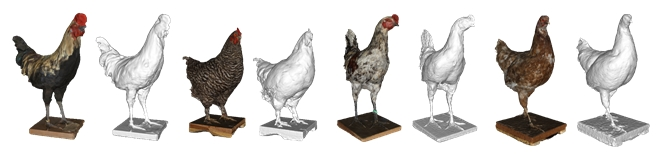
\includegraphics[scale=0.8]{figs/CHICKENS.jpg}}
\caption{Results in the field of 3D reconstruction. The digital models of chickens are obtained using the web-based tool ARC3D. These models were constructed as part of the iMinds INSTANCE project.}
\end{figure}
\section{Related Work}
This section serves to present some of the work done in the field of 3D reconstruction and to discuss its techniques and results in the light of this project.\\
   \\
\linebreak
A list of 3D reconstruction software can be found in appendix A. Most of the entries in this list do not fully reflect the aims of this project either because they make use of 3D scanners or other specialized hardware or because they don't provide support for automatic modeling. Nonetheless, the accuracy with which such software reconstructs an object is an important factor to consider when deciding whether this project should be considered a success.\\
\linebreak
Out of the software presented in appendix A, the tool which best resembles the aims of this project is Ku Leuven's ARC3D\footnote{\url{http://homes.esat.kuleuven.be/~visit3d/webservice/v2/}}. This impressive web-based software is a free, fully-automatic tool for extracting a 3D model from a sequence of images. Its 3D photo gallery\footnote{\url{http://homes.esat.kuleuven.be/~konijn/3d/}} unveils a series of life-like models, some of which were even used in order to print replicas of the initial object.\\
\linebreak
ARC3D bases its computation on the notion of dense reconstruction\cite{tingdahl_lncs_11}. This is more powerful than the approach described in the following chapters of this document because it aims to estimate the depth of the scene at every pixel of the image, not only at a few relevant locations. Albeit dense reconstruction leads to better results, the risks involved in understanding, planning and implementing it in time make it an unfeasible approach for the core of this project. Due to the use of sparse reconstruction, the results of this project are expected to be noisier than those of ARC3D. 


\chapter{Preparation}
The original aims of this project, as presented in the project proposal, amount to a very broad description of the task to be undertaken. However, the successful completion of a challenging project of this scale requires a great deal of careful planning. This chapter presents some of the aspects which factored into planning the execution of a system which aims to reconstruct the scene from a sequence of images.\\
\linebreak
The chapter starts off by identifying the requirements of the system, then it proceeds to describe the structure of the project as it has developed from these requirements. What follows is a description of the tools and methodologies involved in the development of this project. 

%\subsection{Stereo vision and stereo correspondence}
%Stereo vision is the process of recovering depth information from a pair of 2D %projections of the a scene as seen from two different viewpoints.\\ 
%\textit{Although in this project more than two viewpoints will be used, the task of recovering 3D data from multiple 2D projections is difficult for the same fundamental reason as stereo vision is. For simplicity, this section will analyze the difficulties which arise from attempting to recover a 3D scene from two images.} \\

\section{System Overview and Requirements Analysis}
This section aims to identify the requirements which must be fulfilled by any successful implementation of the system described in this document.\\
In addition to serving as a criterion in deciding whether the project is successful or not, such an analysis is an inherent part of the early stages of the project because it provides a base for planning the implementation and for structuring the system.\\
\linebreak
This section presents a broad overview of the system and then proceeds to identify the functional requirements of the project.
\subsection{Overview of the Project}
In order to achieve the purposes of this project, a working system which constructs a three-dimensional model based on a sequence of images must be put together. \\
After analyzing the input images, the system aims to build a set of points which are considered to be lying on the surface of the input object. These points are then connected together in order to construct a polygon mesh. The newly-constructed surface is then exported as a \textbf{PLY} file.\\

\subsection{Functional Requirements}
\begin{samepage}
Table 2.1 summarizes the goals of this project. The information displayed in this table is in conformity with what was presented in the project proposal, but it provides a lower-level overview of the functional components of the system.\\
For each of the functional components listed above the table specifies the priority within the system and provides an estimate of the difficulty and risk expected to arise in the implementation of that component. Because there is a substantial amount of risk involved in carrying out this project, careful consideration was given to estimating the risk of each functional unit. The main  factors which were taken into account in determining the risk of a task are:
\begin{itemize}
\item whether the task is ill-posed. For reasons presented in the introductory chapter of this document, the main source of risk in this project comes from the ill-posed nature of the underlying problem.
\item whether the outcome is expected to need further refinement. Post-processing is commonly used in order to correct the result of an error-prone computation.
\item whether it involves solving complicated mathematical equations. I consider this to be a source of risk because typically such computations are harder to debug and imply a loss of precision.
\end{itemize}     
\begin{center}
\begin{table}
\begin{tabularx}{\textwidth}{@{} Y c c c @{}} % use 'Y' for first column
\toprule
\textbf{Functional Requirements} & \textbf{Priority} & \textbf{Difficulty} & \textbf{Risk}\\ \hline
\midrule
Build a tool for generating pictures from a 3D model                    &   High       &     Low      &   Low \\ \hline \addlinespace
Implement a tool which constructs a point cloud using triangulation   &   High       &     Medium      &   High \\ \hline \addlinespace
Improve stereo correspondence using an epipolar filter                  &   Medium       &     High      &   High \\ \hline \addlinespace
(optional)Implement other filters to build a better point cloud         &   Low       &     Medium      &   Medium \\ \hline \addlinespace
Construct the surface from the resulting point cloud                    &   Medium       &     High      &   High \\ \hline \addlinespace
Add functionality to export the surface as .PLY                         &   Low       &     Low      &   Low \\ 
\bottomrule
\end{tabularx}
\caption{Functional requirements} 
\label{table:nonlin}
\end{table}
\end{center}
\end{samepage}
It is important to note that this system only aims to build the polygon mesh of the surface. Therefore I regarded capturing the texture and shading of the scene non-requirement. The system can be extended later to include this functionality.\\
I am also planning to build the system as one or multiple console applications, hence discarding the need to build a user interface. The applications will display a help message containing information about the tool's intended purpose and usage.

\section{The Main Components of the System}
After a careful evaluation of its required functionality, the system was split into these logically-different entities:
\begin{itemize}
\item \textbf{Image Generator}
Given a three-dimensional object as input, the picture generator produces a specified number of digital pictures of that object, along with the corresponding locations from which the pictures have been taken. 
\item \textbf{Point Cloud Constructor}
The point cloud constructor aims to generate points which lie on the surface of the input model in the three-dimensional space. 
\item \textbf{Surface Reconstructor}
The surface reconstructor converts the point cloud constructed by the previous module into a triangular mesh. The resulting representation of the surface is exported into a \textit{.PLY} file.
\item \textbf{Evaluation Module}
The purpose of the evaluation module is to analyze the performance of the point cloud constructor and of the surface reconstructor by comparing their result to the original model. \\
\end{itemize}
\begin{figure}
\centerline{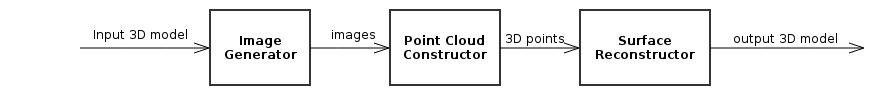
\includegraphics[scale=0.7]{figs/overview.png}}
\caption{An overview of the system}
\end{figure}
 

\section{Dependency Analysis}
To effectively plan the development of the system, I analyzed the dependencies between the functional components identified in the previous sections. Since the image generator and the surface reconstructor have not been decomposed into lower-level units up to this point, this section will focus only on the central part of this project, the point cloud constructor.\\
\pagebreak
Figure 2.2 reveals the high degree of interdependence between the different units of the point cloud construction module. I decided to deal with the intricacies of integrating these units together as early in the development as possible by implementing a very primitive first prototype. This prototype doesn't contain any filters or cloud exporters and it only imports two images whose corresponding camera matrices are known. This approach is a good fit for this project because it decouples the complex integration of units from the implementation of some of the components which carry a greater deal of difficulty or risk. 

\begin{figure}
\centerline{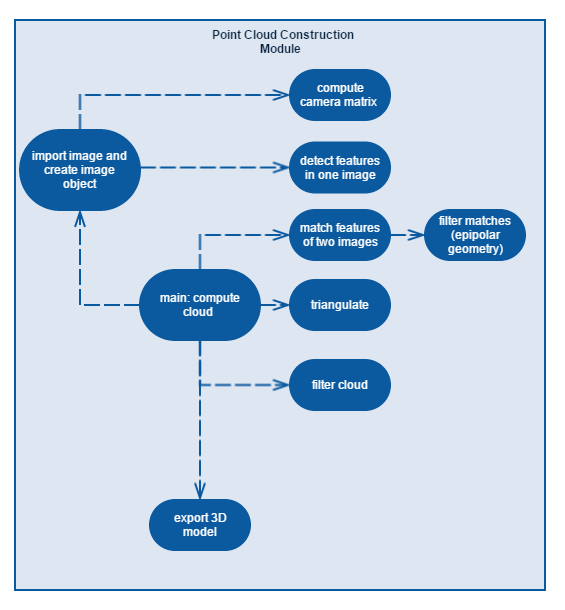
\includegraphics[scale=0.75]{figs/dependencies.png}}
\caption{Dependencies between different units of the point cloud construction module}
\end{figure}


\section{Choice of Tools}

\subsection{Programming Languages}
The main programming language used throughout this project is C++. This choice is motivated by the need to take full advantage of computer vision and computational geometry open-source l7ibraries such as \emph{OpenCV}, \emph{PCL} or \emph{GCAL} which are all written in C++. Another advantage of using C++ for implementing a system which deals with complex computations on images is its characteristic execution speed.\\
I only used C/C++ before in order to implement small practice programs and for implementing the ticks in part IB. Consequently, I needed to adjust to writing C++ programs in an object-oriented fashion and to using features newly introduced in C++11 or in C++14.\\
\linebreak
Python was chosen for implementing the picture generator and parts of the evaluation module. The main reasons for doing so are library availability and the convenience with which one can write small scripts for interacting with C++ binaries.\\
I had no experience with Python before taking on this project.   

\subsection{Libraries and other external software}
As mentioned before, this project relies heavily on libraries which provide working implementations of the tasks considered to be outside the purposes of this project, or just unfeasible to implement from scratch in the given period of time. Figure 2.3 shows the libraries (and the standalone software) which helped bring about the successful completion of the project. The advantages and intricacies which accompanied the use of some of these libraries will be described in more detail in the implementation chapter, where they can be better put into context. The more important ones, however, are introduced in the paragraphs to follow:

\begin{figure}
\centerline{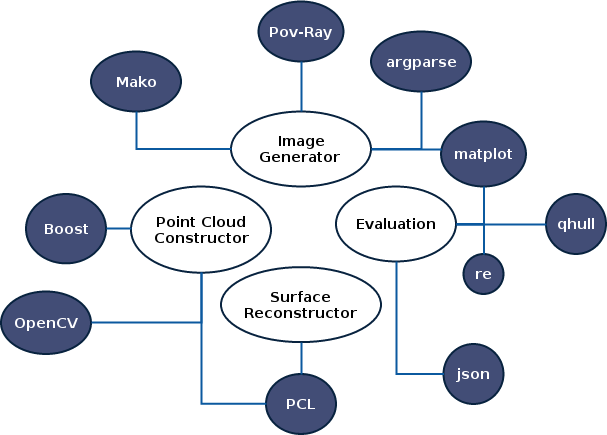
\includegraphics[scale=0.7]{figs/libraries1.png}}
\caption{The libraries and other external software used in the development of this project. The white nodes represent modules of the project.}
\end{figure}
\subsubsection{The Ray Tracer} 
The purpose of one of the main parts of the system, the image generator, is to produce an alternative to photographs of a real-life object. The performance of the system will be evaluated based on what it produces when applied to this computer-generated input. Therefore, for this evaluation to be sound, the input used must be a near photo-realistic representation of the object.\\  
\linebreak
A ray tracer accomplishes just that: given a three-dimensional description of a scene, it creates a digital image of that scene as seen from a predefined location. Many of the ray tracers available yield pictures which are realistic enough for the purposes of this project. \\   
I used \textbf{The Persistence of Vision RayTracer}, or \textbf{POV-Ray}, because it generates images from a text-based scene description. This gives me a lot of flexibility in setting the location of the camera and the light conditions of the scene for every snapshot in turn directly from the script.\\
Another great advantage of \textbf{POV-Ray}\footnote{\url{http://www.povray.org/}} is that it comes with a free object collection (\url{http://objects.povworld.org/}). I can evaluate the results of my system on any one of these instead of having to create my own objects.\\
Convenience factors aside, \textbf{POV-Ray} is one of the highest-quality free ray tracers available.\footnote{\url{http://hof.povray.org/}}

\subsubsection{OpenCV}
A core task of the proposed system is solving the \emph{stereo correspondence problem}\footnote{Stereo correspondence = the problem of determining the corresponding parts between two images}. The most commonly used solution for this problem is the \emph{feature-based} approach:
\begin{itemize}
\item \textbf{detect features:} In each of the two images, find the key locations (or features) which are likely to be relevant in determining a correspondence. In scale-invariant feature detection, the features are defined as the positions of local maxima and minima resulted from convolving the grayscale image with the \emph{Difference of Gaussians} kernel. This operation is performed for a multitude of scale parameters $\sigma$ in order to detect features of different sizes.
\item \textbf{extract feature descriptors:} For each of these features, extract relevant information about the surrounding area which can be used to identify similar feature points.
\item \textbf{match features:} Compute a mapping between two given sets of features (one for each of the views considered) such that the corresponding descriptors of each pair are similar enough to be considered potential solutions for the stereo correspondence problem.
\end{itemize}

\emph{OpenCV} is one of the very few open source computer vision libraries available. Its widespread usage suggests that it is reliable and would make a competent choice for solving the stereo correspondence problem. It provides support for all of the above-mentioned tasks along with an easy-to-use built-in function for visualizing the resulting correspondences.

\subsubsection{PCL}
\emph{The Point Cloud Library}, or PCL\footnote{\url{http://pointclouds.org/}}, contains a vast collection of state-of-the-art algorithms for processing 2D or 3D sets of points. It consists of several modular libraries (filters, surface, kdtree etc.) which have proven useful for improving the results of different parts of this project. The surface reconstruction module, in particular, is heavily reliant on the algorithm for fast triangulation of unordered point clouds\cite{Marton09ICRA} provided by PCL\footnote{\url{http://pointclouds.org/documentation/tutorials/greedy_projection.php}}.

\subsubsection{Qhull}
One of the metrics used in the evaluation module in order to estimate the accuracy of the result is the volume of the convex hull of the resulting point cloud (see the chapter 4).\\
Although constructing a tool for computing the convex hull of a set of 3D points is not a particularly difficult task (my implementation based on Franco Preparata and Ian Shamos's book on computational geometry{Preparata} can be found at \url{https://github.com/ilinca-sorescu/convex-hull}), a more suitable alternative for evaluating the point cloud constructor is to use \emph{qhull}\footnote{\url{http://www.qhull.org/}} instead because it handles the roundoff errors which arise from doing floating point arithmetic and it provides various options for dealing with precision errors in estimating the volume of the resulting convex hull. 

\subsection{The programming environment}
The development was carried out on my personal computer running Arch Linux(rolling release).\\
The programming environment used consists of the \textit{Vim} text editor enhanced with several plug-ins for boosting productivity. The most important of these are \textit{syntastic}\footnote{\url{https://github.com/scrooloose/syntastic}} for highlighting errors directly inside the text editor and \textit{youcompleteme}\footnote{\url{https://github.com/Valloric/YouCompleteMe}} which provides as-you-type semantic code completion.\\
Other command-line tools used for compiling and debugging the code include g++, gdb and the IPython console. The build system used for C/C++ source code will be explored in more detail in the implementation chapter.

\subsection{Version control}
The use of a version control system is crucial for the successful completion of a project of this scale. I used \emph{Git} in order to keep track of the changes that occurred in the source code, configuration files, and in the \LaTeX\  source of this document. The main reasons for choosing this particular version control system are the ease with which it can be coupled with a remote repository and my own experience with it.

\subsection{Backup}
A remote repository was assembled to back up the latest stable version in case of a crash. The \emph{Dropbox} file synchronization service was used to ensure the full recovery of the files which were not tracked by Git. One of the great advantages of this approach to backing up files is that it uploads all of the changes automatically, without having to rely on the user to explicitly do so.  
%\end{minipage}%
%\begin{minipage}{0.2\textwidth}
	%\begin{center}
		%\
\includegraphics[scale=0.18]{figs/gitcat.png}\\ 
		%\vspace{10pt}
%		
\includegraphics[scale=0.1]{figs/dropboxlogo.png}
	%\end{center}
%\end{minipage}
\subsection{Other Tools}
\textit{Meshlab}\footnote{\url{http://meshlab.sourceforge.net/}} and \textit{Geomview}\footnote{\url{http://www.geomview.org/}} were used for  viewing and editing the resulting surface meshes. 

\section{Software Engineering Techniques}
Although the nature of Part II projects promotes the use of the \emph{Waterfall Development Model}, the components of this system which are associated with a high degree of risk would benefit from the rapid prototyping characteristic to \emph{iterative design}. One way to make the most of both paradigms is to adopt the \emph{Incremental Build Model}:\\
\begin{adjustwidth}{0.7cm}{}
The process begins by analyzing the requirements dividing the task into the loosely-coupled modules (or 'builds') defined above (see sections 2.2 and 2.3). Each of the modules go independently through the stages of a waterfall-like model: they are designed, implemented and then tested and evaluated accordingly. If the result of the evaluation is not yet satisfactory for a given build, it will go through all of the stages again until adequate results are achieved.\\
\end{adjustwidth} 
This methodology provides a sensible approach for implementing the proposed system because even though the main objectives are clearly set right from the beginning (thus maximizing the probability of meeting the success criteria) some initially under-specified implementation details are more flexible and can change as a result of the analysis done at the previous iterations. This aids the exploratory nature of the point cloud construction module in particular.  

\section{Summary}
This chapter provided a description of the intended outcome of this project and of the choices made prior to implementation in order to ensure its successful completion. It outlined the main requirements and explained how they were refined into a high-level structure of the system, explained the arguments which sustain the choice of several tools and programming languages and provided a description of a suitable implementation approach.
\chapter{Implementation}

The aim of this chapter is to acquaint the reader with the internal workings of the system by providing an in-depth description of the techniques used in order to add functionality or to improve the accuracy and overall performance of the system.\\
\linebreak
As mentioned in the previous chapter, the system is comprised of four major parts:
\begin{itemize}
\item \textbf{Image Generator}
\item \textbf{Point Cloud Constructor} 
\item \textbf{Surface Reconstructor}
\item \textbf{Evaluation Module}
\end{itemize}
Each of the following sections will focus on one of these modules. 


\section{The Image Generator}
As described in the previous section, this module produces a sequence of digital snapshots of a given three-dimensional object as seen from different locations in space. \\
Perhaps the most important aim of this project is to decide whether it would be practical to implement a low-cost system for creating digital representations of real-life objects based on pictures instead of using three-dimensional scanners. Therefore it might seem a bit odd that such a module is needed at all as it is restricting the system's interaction with the outside world. This section aims to explain why such an input generator is used and provide a detailed overview of its intended usage. 
\subsection{The role it plays in the system}
Complex measurements and calculations must be performed in order to determine the accuracy with which the output of the system resembles the real-life object used as input. To avoid this complexity, the input of the system was changed from a sequence of photographs of an object acquired using a hand-held camera to a sequence of digital snapshots of a preexisting three-dimensional model. This is a natural first-step to be taken in deciding whether such a system would yield a reliable representation because it enables one to evaluate the results by comparing the output directly to the input model. More on this topic in the evaluation chapter.\\
Here are some additional advantages of using digital snapshots instead of photos: 
\begin{enumerate}
\item there is no need to worry about camera calibration.
\item the configuration of the scene is very easy to change (e.g.\ the location and orientation of the light sources, the number of snapshots taken, etc.). This is a very important advantage in determining the limiting conditions in which the output is accurate.
\item the input generator can produce a lot of snapshots effortlessly and record the locations from which they were taken.
\item no human assistance is needed in evaluating the system.
\end{enumerate}
The system can be extended to take real photographs as input simply by adding a calibration module.

\subsection{Usage}
This module is executed as a console application. The user must specify the following arguments:
\begin{itemize}
\item \textbf{Filename} The name of (and relative path to) the input object. This must be an include file for \textbf{The Persistence of Vision Raytracer (POV-Ray)} and have the extension \textit{.inc}. The input file is assumed to meet the conditions outlined below:
	\begin{enumerate}
		\item the file defines only one object.
		\item the object defined is included in the scene. For better results it should be placed in the vicinity of the origin.
		\item the scene defined in the file mustn't contain any lights or cameras.
		\item no run-time errors are produced as a result of attempting to render the file using \textbf{POV-Ray}. 
		\item the file doesn't contain any instruction whose purpose is to redefine the length of the units used to something other than the standard \textbf{POV-Ray} units. 
	\end{enumerate}    
\item \textbf{N} The number of snapshots to be taken. This can be any integer greater than 3.
\item \textbf{R} The radius of the sphere considered. The following condition must be fulfilled by \textbf{R}: If you were to look towards the origin through air (using no distorting lenses) from any point at a distance \textbf{R} from the origin you would see the whole object. Here, the origin refers to the origin of the \textbf{POV-Ray} coordinate system and the distance is measured in \textbf{POV-Ray} units.  (for more details on the \textbf{POV-Ray} coordinate systems see \url{http://www.povray.org/documentation/view/3.6.1/15/})
\item {folder} The destination folder.
\end{itemize}

\subsection{Language and Libraries}
The image generator was implemented using Python. The main factor involved in this decision was the availability of a lightweight library for dealing with templates. I used \textbf{Mako} (\url{http://www.makotemplates.org/}) in order to create \textit{.pov} files from the template \textit{povTemplate.mako}: 

\begin{verbatim}
#include "${filename}"
#include "colors.inc"

light_source { <100, 100, 100> color rgb<1, 1, 1> }

camera {
          location <${", ".join(str(x) for x in camera)}>
          look_at <0, 0, 0>
       }
\end{verbatim} \\

\textbf{Mako} enables the programmer to control the value of the variables (marked with \$) from the Python script. \\
The \textit{.inc} file which defines the input model is included in the first line of the template. \\
I chose to use this approach because it is a painless and straightforward way to control the location of the camera and the light conditions of the scene regardless of the input model used. 

\subsection{Effect and Output}
Given the name of the input file, the number of snapshots to be produced(\textbf{N}) and the radius of the sphere considered(\textbf{R}), the image generator determines \textbf{N} points uniformly distributed on the surface of the sphere of radius \textbf{R} centered in origin. These \textbf{N} points represent the locations from which the snapshots will be taken. For each of these camera locations a new \textit{.pov} file will be generated from the \textbf{Mako} template as described in the previous section. Note that the camera is always pointing towards the origin. \\
The \textit{.pov} files are rendered using \textbf{POV-Ray} to create the desired snapshots.


\begin{figure}
\centerline{\includegraphics[scale=0.58]{figs/basic_proto.png}}
\caption{Overview of the basic prototype of the point cloud constructor: the two images are imported and their corresponding \emph{Image} objects are constructed. These objects are then passed on to the \emph{Feature matcher} which finds corresponding locations between them. For each of these point correspondences, \emph{triangulation} is called to determine the world coordinates of the 3D point rendered at both image locations. The result is then added to the cloud.}
\end{figure}

\section{The Point Cloud Constructor}
Given a sequence of snapshots, the point cloud constructor finds correspondences between pairs of snapshots and uses these correspondences to determine the three-dimensional position of points located on the surface of the object. \\
\linebreak
As specified in the preparation chapter, a primitive prototype has been implemented early on in the development of the system. This section starts by presenting the principles and techniques used for implementing this basic prototype, then it proceeds to explain the measures which were taken to improve on these early results.

\subsection{A Basic Prototype}
A prototype was assembled to integrate primitive implementations in order to fulfill the main functional requirements which are part of the point cloud constructor. This prototype is characterized by its disregarding of accuracy. It attempts to create a reconstruction from only two input images. \\
Figure 3.1 gives an outline of the computation.

\subsubsection{Importing the Images}
For each of the snapshots used as input a correspondent instance of the \emph{Image} class is created. These instances contain the relevant information characteristic to a single view:
\begin{itemize}
\item The location (in world coordinates) of the center of the camera. This is information is provided by the image generator.
\item The features and descriptors. The \emph{OpenCV} interfaces \emph{FeatureDetector} and \emph{DescriptorExtrator} define easy-to-use methods for dealing with these.
\end{itemize}

\begin{figure}
\centerline{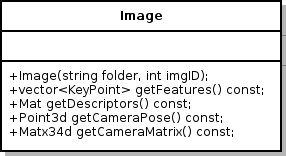
\includegraphics[scale=0.6]{figs/image.png}}
\caption{The public methods of the \emph{Image} class.}
\end{figure}

In a later prototype, the \emph{Image} class will be extended further to include the camera matrix. In this respect, the basic prototype is structured differently because it makes use of the simplifications which arise from having only two views. The reasons for this change will be presented later in this chapter.

\subsubsection{The Camera Matrix}
In computer vision a \emph{camera} is defined as a mapping from a 3D space (the object space) to a 2D space (the image)\cite[p.153]{Hartley+2003}.\\ The camera model used throughout this project is the \emph{basic pinhole camera model}.
\begin{figure}
\begin{center}
\tdplotsetmaincoords{70}{110}
\begin{tikzpicture}[tdplot_main_coords]

\draw[thick,->] (0,0,0) -- (3,0,0) node[anchor=north east]{$x$};
\draw[thick,->] (0,0,0) -- (0,7,0) node[anchor=north west]{$z$};
\draw[thick,->] (0,0,0) -- (0,0,3) node[anchor=south]{$y$};
\node at (0,0,0) {\textbullet} ;
\node at (0,-0.5,0) {O};
\draw[thick] (0,0,0) -- (2, 7, 2.5) ;

\draw[thick] (0,5.4,0) node{\textbullet} node[anchor=north west]{P} -- (2, 7, 2.5) node{\textbullet}  node[anchor=south west]{\bf{X}};

\coordinate (Shift) at (0,3,0);
\tdplotsetrotatedcoordsorigin{(Shift)}

\draw[thick,tdplot_rotated_coords, ->] (0,0,0) -- (2,0,0) node[anchor=north east]{$x$};
%\draw[thick,tdplot_rotated_coords, ->] (0,0,0) -- (0,1,0) node[anchor=north west]{$z$};
\draw[thick,tdplot_rotated_coords, ->] (0,0,0) -- (0,0,1.25) node[anchor=south]{$y$};

\node[tdplot_rotated_coords] at (0,0,0) {\textbullet} ;
\node[tdplot_rotated_coords,anchor=south west] at (0,0,0) {Q};

\draw[thick, tdplot_rotated_coords] (0,0,0) -- (-1,0, 0.5) node{\textbullet} node[anchor= south west]{\bf{y}};
\draw[thick,tdplot_rotated_coords] (3.5, 0, 2) -- (3.5, 0, -1.5);
\draw[thick,tdplot_rotated_coords] (3.5, 0, -1.5) -- (-3.5, 0, -1.5);
\draw[thick,tdplot_rotated_coords] (-3.5, 0, -1.5) -- (-3.5, 0, 2);
\draw[thick,tdplot_rotated_coords] (-3.5, 0, 2) -- (3.5, 0, 2);
\end{tikzpicture}
\caption{The pinhole camera model: X(in the object space) is represented in the image at location y(in image coordinates).}
\end{center}
\end{figure}
In this model, the camera is placed at the origin, facing the positive z-axis (also referred to as the principal axis). The image plane is at a distance \emph{f} in front of the camera, perpendicular to the principal axis. This camera maps points from the object space to the intersection between the image plane and the line connecting the origin to that point. This set-up is depicted in Figure 3.2.\\
\linebreak
The relation between 3-space and 2-space, as defined by the pinhole camera, can be easily modeled using the 3X4 camera matrix $\mathbf{C_{0}}$: 
\begin{equation}
\mathbf{y = C_{0}X}
\end{equation}
In this equation \textbf{X} and \textbf{y} are the homogeneous coordinates of the point in object space and its correspondent in the image plane respectively.\\
For the basic pinhole camera model, the camera matrix $\mathbf{C_{0}}$ is:
\[ \mathbf{C_{0}=\left(\begin{array}{cccc}
f & 0 & 0 & 0 \\
0 & f & 0 & 0 \\
0 & 0 & 1 & 0\end{array} \right)}\] 
Assuming that $f = 1$, $\mathbf{C_{0}} = \left ( \begin{array} {c|c} \mathbf{I} & \mathbf{0} \end{array} \right )$
\\
\linebreak
More often than not, the 3D locations are not specified in a camera-centric coordinate system but in an arbitrary one, in world coordinates. A more general form of equation (3.1) relates $y$ to $X'$, the correspondent in homogeneous world coordinates of point $X$:
\begin{equation}
\mathbf{y = CX'},\hspace{20pt} \mathbf{C} = \left ( \begin{array} {c|c} \mathbf{R} & \mathbf{t} \end{array} \right )\\
\end{equation} where $\mathbf{R}$ is a 3x3 rotation matrix and $\mathbf{t}$ is a translation column vector. For the derivation of equations 3.1 and 3.2 from basic principles of the pinhole camera model see Appendix C.\\

\subsubsection{Using OpenCV to Find the Camera Matrix}
\cite[p.~129]{baggio2012mastering}

\subsubsection{Triangulation}
The term \emph{triangulation} denotes the process of determining the third vertex of a triangle by means of intersecting two of the lines which form the edges of the triangle.\\
This section follows the process of intersecting the rays back-projected from a pair of matching image coordinates, $p1=(u, v)$ and $p2=(u', v')$, in order to determine the location of the 3D point $X$ which is depicted in both of these image locations.\\
\linebreak
The \textbf{Linear-LS}\cite[p.~8]{Hartley96triangulation} method for solving the triangulation problem boils down to solving the system of equations:
\begin{equation}
\mathbf{AX} = \mathbf{B} 
\end{equation}
where \textbf{A} and \textbf{B} are defined as follows:
\begin{verbatim}
  Matx43d A(p1.x*C1(2, 0)-C1(0, 0), p1.x*C1(2, 1)-C1(0, 1), p1.x*C1(2, 2)-C1(0, 2),
            p1.y*C1(2, 0)-C1(1, 0), p1.y*C1(2, 1)-C1(1, 1), p1.y*C1(2, 2)-C1(1, 2),
            p2.x*C2(2, 0)-C2(0, 0), p2.x*C2(2, 1)-C2(0, 1), p2.x*C2(2, 2)-C2(0, 2),
            p2.y*C2(2, 0)-C2(1, 0), p2.y*C2(2, 1)-C2(1, 1), p2.y*C2(2, 2)-C2(1, 2));

  Matx41d B(-p1.x*C1(2, 3)+C1(0, 3),
            -p1.y*C1(2, 3)+C1(1, 3),
            -p2.x*C2(2, 3)+C2(0, 3),
            -p2.y*C2(2, 3)+C2(1, 3));
\end{verbatim}
Here, \textbf{C1} and \textbf{C2} are the camera matrices of the two views considered.

\begin{proof}
Using equation 3.2 and the homogeneous form of $p1$: \\
\begin{center}
$\begin{bmatrix}
	uw \\
	vw \\
	w \\
  \end{bmatrix} = \textbf{C}_{1}\textbf{X}$
\end{center}
This is equivalent to:
\begin{center}
$\systeme*{
uw = \textbf{c}_{1}^T \textbf{X},
vw = \textbf{c}_{2}^T \textbf{X},
w = \textbf{c}_{3}^T  \textbf{X}}$
\end{center}
where  $\mathbf{c}_{i}^T$ of $\mathbf{C}_{1}$ is the $i^{th}$ row of $\mathbf{C_{1}}$. \\

By substituting w from the last equation the system becomes:
\begin{center}
$\systeme*{
u * \textbf{c}_{3}^T \textbf{X} = \textbf{c}_{1}^T \textbf{X},
v * \textbf{c}_{3}^T \textbf{X} = \textbf{c}_{2}^T \textbf{X}}$ \\
\end{center}
\begin{center}
$ => \begin{cases}
(u * \mathbf{c}_{3}^T - \mathbf{c}_{1}^T) \mathbf{X} = 0  \\
(v * \textbf{c}_{3}^T - \mathbf{c}_{2}^T) \mathbf{X} = 0
\end{cases}$
\end{center}

Equivalent equations can be obtained by using \textbf{p2} and \textbf{C2}. Together they form the following system of equations:
\begin{align}
	\textbf{A'}\textbf{X} &= \textbf{0}\\ 
\textbf{A'} &= \begin{bmatrix}
u * \mathbf{c}_{3}^T - \mathbf{c}_{1}^T\\
v * \mathbf{c}_{3}^T - \mathbf{c}_{2}^T\\
u' * \mathbf{c'}_{3}^T - \mathbf{c'}_{1}^T\\
v' * \mathbf{c'}_{3}^T - \mathbf{c'}_{2}^T
\end{bmatrix}
\end{align}

After forcing \textbf{X} to be of the form 
$\begin{bmatrix}
x \\
y \\
z \\
1
\end{bmatrix}$ and then eliminating the now superfluous column of \textbf{A}, the system of equations becomes:
\begin{center}
	\textbf{A}\textbf{X} = \textbf{B}
\end{center} for the \textbf{A} and \textbf{B} defined above.
\end{proof}
Since \textbf{A} is not invertible its pseudo-inverse must be computed in order to determine \textbf{X}. The function \emph{invert} from \emph{OpenCV} provides an easy way to deal with computing the pseudo-inverse of non-quadratic matrices by using the \emph{singular value decomposition}\cite[p.~82]{Suli+2003} factorization method.\\
\linebreak
Although suitable for a basic prototype, the solution for the triangulation problem described in this section is generally not recommended for constructing a projective reconstruction. Its main shortcoming comes from its inability to deal with noise: a central assumption made by this method is that the two rays will intersect. Albeit this should be the case in ideal conditions, it is not generally true of two lines laying in 3-space. Since any amount of noise could cause the two rays to meet at infinity, a more error-resilient approach should be adopted. Such a method will be presented later in this chapter.


\subsection{Multiple-View Reconstruction}
The techniques described so far assumed the use of only two input images. This section stands to identify the intricacies which arise from constructing a 3D model from multiple views and to present a solution for this type of reconstruction.

\subsubsection{Camera Matrix for a "Look-at" Camera}
Thus far, the point cloud constructor yielded an up-to-scale representation of the input object. This has to do with the way in which the camera matrix is constructed: the first view is implicitly associated with the canonical camera matrix; the camera matrix for the second view is then determined in relation with the camera pose for the first view. The camera matrices computed this way are interdependent, and they introduce a scaling factor associated with each pair of images. This becomes problematic when the reconstruction is made from more than two images because each individual pair will give raise to a different scaling factor. \\
This section presents a method of deducing the camera matrix directly from the camera pose and the viewing direction.

\subsubsection{The Reconstruction Approach}
\begin{figure}
\begin{center}
\includegraphics[scale=0.6]{figs/minRatio.png} 
\caption{Motivation for minRatio: C1 and C2 are the locations of the camera for two different images. An object gets rendered in the second image at location \emph{x}. When an error (in red) in determining the position of \emph{x} is introduced, it results in a distance equal to the magnitude of the segment (object, P) between the real and computed 3D coordinates of the object. This distance increases dramatically when C2 is placed very close to C1. The two red segments have the same length and C2'x = C2x.}
\end{center}
\end{figure}
As is case of stereo vision, 3D reconstruction is performed by determining similarities between a pair of images in order to infer the depth at various locations in the scene. When more than two images are provided, the result consists of the points determined by analyzing multiple pairs. The ideal method of selecting pairs of images from a set maximizes the number of matching features taken into account, while avoiding to pair up dissimilar images which are more likely to generate erroneous data.\\
\linebreak
Initially every image was paired with its K-closest neighbors. Empirical evidence suggested that if the two images were taken from a very close distance to each other the generated noise increased dramatically. Figure 3.4 illustrates why this is the case. \\
In light of these observations a new method was proposed: two images are paired together only if the distance between the cameras belongs to the interval $[minRatio \cdot R, maxRato \cdot R]$, where $minRatio$ and $maxRatio$ are two parameters whose default values are 0.04 and 0.65 and $R$ is the radius of the sphere from which the pictures were taken (the distance from the position of the camera to the origin).

\subsection{Refining the Reconstruction and Improving Performance}
As mentioned right from the beginning of this document, the proposed system was expected to be highly error-prone. Consequently, a software engineering paradigm which allowed for repeatedly adding improvements to the initial design has been employed. This section aims to analyze these improvements.
\subsubsection{Epipolar Filtering}
Unlike the other improvements described in this section, the epipolar filtering is critical to an accurate reconstruction. The reason why it is not considered to be part of the basic prototype described above is that epipolar filtering is not essential to the integration of the main components of this module. In contrast, it adds a great deal complexity to what was designed to be a simple first iteration in the incremental development model.\\
\begin{figure}
\begin{center}
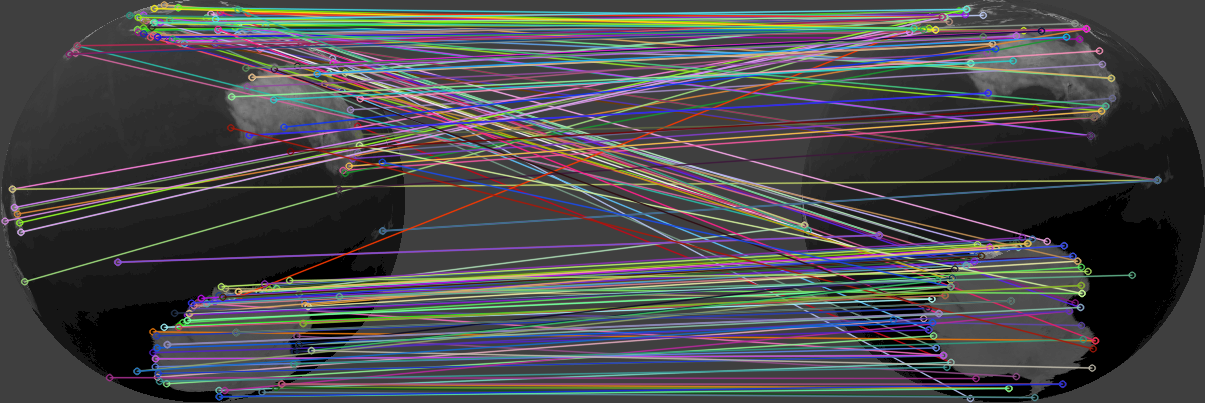
\includegraphics[scale=0.35]{figs/before_epi.png} \\
\vspace{5pt}
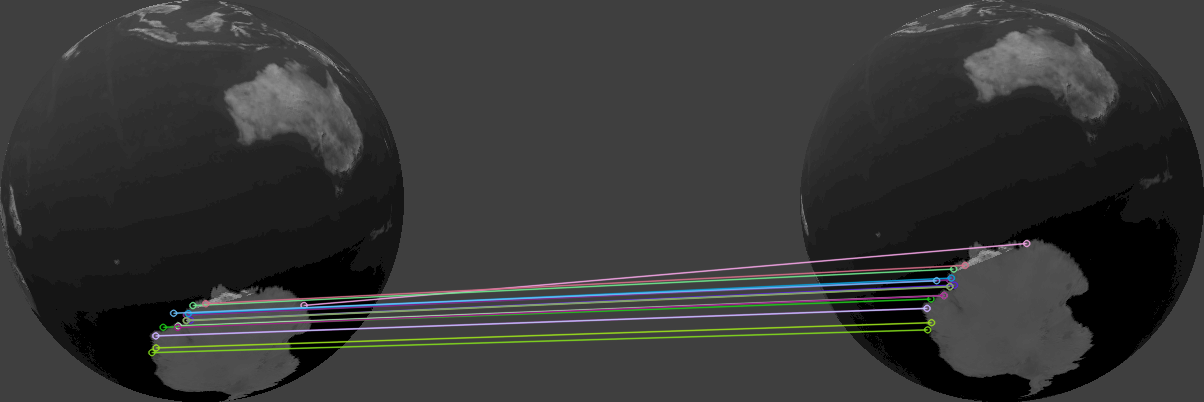
\includegraphics[scale=0.35]{figs/after_epi.png}	
\caption{Before and after epipolar filtering}
\end{center}
\end{figure}\\
Epipolar geometry is the geometry of two views. It aims to describe, for any position in the first view, the region in the second view where its corresponding position might reside. In this project, this knowledge is used in order to detect which of the presumably matching pairs returned by the feature matcher make geometric sense. Figure 3.3 seeks to give the reader an impression of the vast percentage of erroneous correspondences identified by the feature matcher.\\
\linebreak
As depicted in Figure 3.4, each point in one view corresponds to a line in the second view. This means that a location $r$ in the right view is considered to be a correct match for the point $x_{L}$ for any $r$ on the epipolar line. Since it can only ever make sense for $x_{L}$ to get coupled with a unique $r$, this proves that epipolar filtering does not identify all of the erroneous matches. Instead, it reduces the state of possible solutions from a 2 dimensional one (the entire view) to just one dimension (the epipolar line). Figure 3.4 portrays the remaining uncertainty by showing the multitude of points in the object space ($X$, $X_{1}$, $X_{2}$ etc.) which will be projected onto the same point in the left view. The epipolar line is formed by projecting this infinite set of points onto the right view.\\
\linebreak
What follows is a description of some of the key notions pertaining to epipolar geometry \cite[chapter~9]{Hartley+2003}:
\begin{itemize}
\item {\bf{The epipolar plane:}} The rays back-projected from the two corresponding image locations intersect at $X$, the location in the object space whose image is created at $x_{L}$ and $x_{R}$. Therefore, the two rays are coplanar, forming the epipolar plane.  
\item {\bf{The baseline:}} the line joining the camera centers, $O_{L}$ and $O_{R}$.
\item {\bf{The epipole:}} the location in one view which corresponds to the camera center of the other view. It is located at the intersection between the baseline and the image plane. 
\item {\bf{The epipolar line:}} the intersection between the epipolar and image planes. 
\end{itemize}

\begin{figure}
\begin{center}	
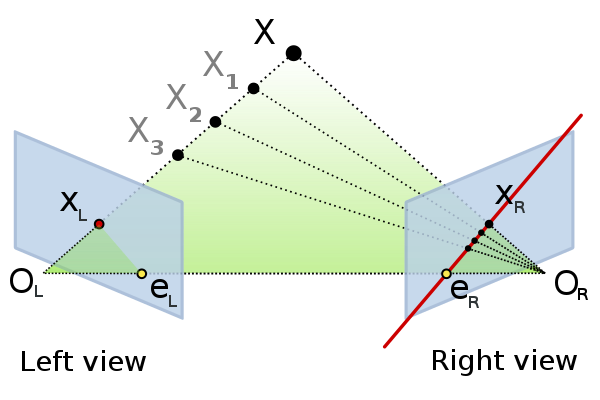
\includegraphics[scale=0.7]{figs/Epipolar_geometry.png}
\caption{Epipolar geometry: this figure illustrates (in red) the epipolar line, or the space of possible correspondences in the right view of point $x_{L}$ in the left view. $O_{L}$ and $O_{R}$ are the locations of the two cameras; $e_{L}$ and $e_{R}$ are the two epipoles. The epipolar plane is featured in green and the two image planes in light blue.}
\end{center}
\end{figure}
 
The following equations illustrate the method used to verify whether two 2D locations, $x_{L}$ and $x_{R}$, could be depictions of the same 3D point. The method assumes prior knowledge of the camera centers, $O_{L}$ and $O_{R}$, along with their corresponding camera matrices, $C_{L}$ and $C_{R}$:\\
\linebreak
\begin{adjustwidth}{0.7cm}{}
The camera matrix relates any point in the object space to a point in the view. By definition the epipole is the image of the camera center of the other view. Therefore, the following equation holds:
\begin{equation}
\mathbf{e_{R} = C_{R} O_{L}}
\end{equation}
\linebreak
Equation 3.4 defines another point which resides on the epipolar line. In addition to $e_{r}$, this point completely determines the space of points in the second view which might correspond to $x_{L}$:
\begin{equation}
\mathbf{p_{R} = C_{R} C_{L}^{\dagger} x_{L}}
\end{equation}
Here, $C_{L}^{\dagger}$ refers to the pseudo-inverse of $C_{L}$. This obeys the equation $C_{L} C_{L}^{\dagger} C_{L} = C_{L}$. 
\linebreak
To show that $p_{R}$ is located on the epipolar line, it suffices to show that $X' = C_{L}^{\dagger} x_{L}$ belongs to the ray back-projected from $x_{L}$:\\

\begin{proof} 
\begin{align}
C_{L}X' &= C_{L} (C_{L}^{\dagger} x_{L})\\
		&= C_{L} C_{L}^{\dagger} (C_{L} X)\\ 
		&= C_{L} X\\
		&= x_{L} \qedhere
 \end{align}
\end{proof}


$x_{R}$ can match $x_{L}$ only if it belongs to the line joining $e_{R}$ and $p_{R}$. To account for the errors introduced by floating point computations, the epipolar test checks whether $x_{R}$ is at a distance of at most \emph{tolerance} away from the epipolar line. The value of \emph{tolerance} can be specified by the user, and it has a default value of 0.0001.   
\end{adjustwidth}

\subsubsection{Other Filters}
There are multiple sources of errors introduced by the computation described so far (e.g.\ the pseudo-inverse of a non-square matrix, the use of a \emph{tolerance} parameter in determining whether a point is part of the epipolar line, floating point arithmetic etc.). Although typically each of these accounts only for an error of up to 0.0001 in the relevant quantities, triangulation can greatly amplify this effect: any amount of error in the estimated location of a 2D feature can lead to a significant difference in the perceived depth of the 3D point found by triangulation and the real location of the feature.\\
Since there is no reliable way to test whether a perceivable error has been introduced, the following measures were taken to remove from the cloud the points which are less likely to be part of a correct representation:
\begin{itemize}
\item \textbf{Statistical Outlier Removal}: For every point in the cloud the mean distance to its K-nearest neighbours is computed. The distribution of these mean distances is assumed to be Gaussian. A point is removed from the cloud if its corresponding mean distance lays outside of a certain interval of the underlying Gaussian.  
\item \textbf{Radius Outlier Removal}: A point is removed from the cloud if there are fewer than \emph{N} points at a distance of at most \emph{d} from the initial point. 
\end{itemize}
Both of these filters are provided by \textbf{PCL}. My implementation is based on the tutorials found at \url{http://pointclouds.org/documentation/tutorials/statistical_outlier.php} and \url{http://pointclouds.org/documentation/tutorials/remove_outliers.php}.\\
\linebreak
Another filter was assembled to limit the magnitude of the error introduced by the use of pseudo-inverses in \emph{Triangulation}: whenever a 3D point is determined, it is re-projected onto the image plane with the use of the camera matrix. If the distance between the feature used in determining the 3D point and the corresponding reprojection is greater than \emph{MaxReprojectionError}, the 3D point is not added to the solution set. 

\subsubsection{Error-resilient Triangulation}
As mentioned above, triangulation consists of solving a system of equations of the form:\\
\begin{center}
$u * \mathbf{c}_{3}^TX - \mathbf{c}_{1}^TX=0$
\end{center}
For noisy data it might be the case that not all of the equations can become equal to 0. The more general form is this:
\begin{center}
$u * \mathbf{c}_{3}^TX - \mathbf{c}_{1}^TX=\epsilon_u$
\end{center}
It is important to note that in dealing with the errors resulted from triangulation, $\epsilon$ is not the value to be minimized. Instead, the measure of error is defined as the error found by reprojecting X onto the image plane:
\begin{center}
$\delta _u = u - \mathbf{c_1X/c_3X}$
\end{center}
\textbf{Iterative-LS}\cite[p.~9]{Hartley96triangulation} aims to  $\delta$
reweigh triangulation until errors are reduced or for at most 10 iterations.
starts off by doing the naive triangulation (corresponding with weights 1 1 1 1)

\subsubsection{Parallelism}
The process of determining points on the surface of the object is computationally expensive. Fortunately, several tasks can be performed in parallel to make full use of the CPU resources available. \emph{Boost} provides a convenient way to deal with parallelism: \\
\begin{verbatim}
 mutex push_backMutex;
 boost::basic_thread_pool pool(8);
 for(auto p1 = 0u; p1 != images.size(); ++p1)
    pool.submit([this, p1, radius, &points3D, &push_backMutex]() {
    	...
    	for every image p2 such that (p1, p2) are a pair:
    		 determine 3D points from analyzing correspondences between p1 and p2
    		 and add them to the solution vector.
    	...
    });
 pool.close();
 pool.join();
\end{verbatim}
The \emph{push\_backMutex} is used to ensure that no two threads attempt to add a solution to the $point3D$ vector at the same time.\\
Thread pools are used on multiple instances across the point cloud construction module. The most notable occasions are the one presented above, and the one involved in reading the input images.

\subsection{Data structures}
Matrix arithmetic is extensively used throughout this module. \\
\linebreak 
\\
\linebreak 

\subsection{The Build System}
By virtue of being the most complex module of the system, the point cloud constructor soon began to span over 10 source files and to have several dependencies. As a result, readjusting the \emph{Makefile} for every new insertion became a burdensome task. The preferred alternative was to use an open-source software construction tool, \emph{Scons}\footnote{\url{http://www.scons.org/}}, which provides built-in automatic dependency analysis. The configuration script for \emph{Scons} was substantially easier to maintain. An example of such a configuration script can be found in Appendix B.

\subsection{Usage}
This module is implemented as an individual console application. The user must specify the path to the folder containing input pictures. The following parameters are optional:
\begin{itemize}
\item \textbf{N}: the number of snapshots to be considered. By default this is equal to the number of images in the specified folder. 
\item \textbf{Conf}: the path to a text file which contains the desired values for \emph{MinRatio, MaxRatio, Maximum reprojection error}, \emph{Tolerance} and the name of the output file.
\end{itemize}

\section{The Surface Reconstructor}


\section{The Evaluation Module}
This module consists of independent pieces of code which serve the purpose of evaluating the performance of the other modules. It is used in order to automatically plot the accuracy of the outcome gathered by varying the input arguments of the point cloud constructor.\\
\linebreak
\textbf{The Data Gatherer} runs point cloud constructor for a specified range of parameters. It exports the generated \emph{config} file along with the output of the point cloud constructor and the timing information obtained by running the \emph{time} command. The name of the \emph{config} file is chosen at random to avoid name clashes.\\
\linebreak
\textbf{Plot Maker} imports the \emph{config} files exported by the data gatherer, and converts them into dictionaries of the form: \begin{verbatim}    
          { 'minRatio':minRatio,
            'maxRatio':maxRatio,
            'reprojectionError':reprojectionError,
            'tolerance':tolerance,
            'outputFilename':outputFilename,
            'inputFolder':inputFolder,
            'numPics':numPics,
            'configFilename': filename }
\end{verbatim}
The dictionaries are filtered to match the purposes of the plot. Typically one of the input parameters is unset such that it can be used as the domain of the function to be plotted.\\
For every value in the domain, some computation is performed on the output of point cloud constructor to evaluate the result at that point in the function. If the computation is thought to be expensive, the resulting data is serialized and dumped on the disk to avoid the need to recompute it. The function is then plotted using \emph{matplotlib}.\\
\linebreak
The evaluation module provides the support for constructing virtually any plot which has to do with the output of the previous modules. The specific metrics and statistical methods involved in evaluating the results will be described further in chapter 4. 
\section{Summary} 


\chapter{Evaluation}
\section{General Results}

\section{Accuracy of Reconstruction}
\subsection{Methodology}
\subsection{Error Metrics}
\subsection{Confidence Intervals}
\subsection{Volume of Reconstruction}
\begin{figure}
\begin{center} 
\includegraphics[scale=0.7]{figs/minRatio0.png}	
\caption{bla}
\end{center}
\end{figure}

\begin{figure}
\begin{center}
\includegraphics[scale=0.7]{figs/volumeByMinRatio.png}	
\caption{lala}
\end{center}
\end{figure}

\begin{figure}
\begin{center}
\includegraphics[scale=0.7]{figs/minRatio004.png}	
\caption{lala}
\end{center}
\end{figure}

\section{Performance Analysis}
\begin{figure}
\begin{center}
\includegraphics[scale=0.7]{figs/time.png}	
\caption{lala}
\end{center}
\end{figure}
\begin{figure}
\begin{center}
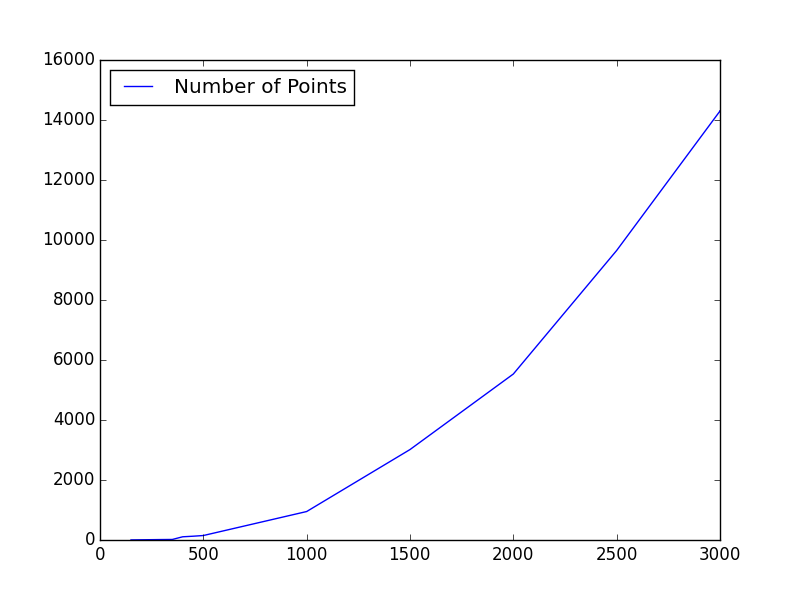
\includegraphics[scale=0.7]{figs/numVertices.png}	
\caption{lala}
\end{center}
\end{figure}

\section{Testing}

\section{Summary}

\chapter{Conclusion}


\section{Achievements}
All of the objectives set in the project proposal had been achieved: a working system for deducing the shape of an object from a sequence of images has been designed, implemented and thoroughly evaluated and tested.\\
\linebreak
This is the largest project I have undertaken, and it allowed me to gain insight into the fascinating fields of computer vision and multiple-view geometry. 

\section{Lessons Learned}
This project enabled me to further my knowledge and skills and I have leaned many valuable lessons throughout. One of the most valuable ones has to do with the importance of planning for failure and allowing time to improve the results. The results from the early stages were rather daunting especially since understanding several research-level techniques and deciding which of the many approaches available in the literature to choose took longer than expected and, in some cases, ended up producing disappointing results. The project would not have been a success had I not chosen an incremental implementation technique and planned for time to go through multiple iterations.\\
\linebreak
Another important lesson I took away from this experience is that the libraries chosen to provide a core functionality do not always come through, or, at least,  not at the expected quality. Perhaps the best example of this is relying on PCL to automatically construct a surface from the point cloud. I spend vast amounts of time trying to improve its performance both by reducing the noise in the point cloud and trying different filtering, resampling and normal estimation methods provided by PCL but with no use. Had I known earlier that this would be the case, I might have chosen a semi-automatic approach similar to the one described in the \emph{Proteus}\cite{ProteusInteractiveSFM} project.
\section{Future Work}
Although the system is complete in the sense that it fulfills the initial objectives, future work can be done to improve the results and to turn this system into a deliverable piece of software. \\
\linebreak
Even though the accuracy of the representation was found to be adequate, the number of input images necessary to produce a satisfactory result is rather disappointing. Future work would focus on reducing the number of images to at most 20.\\ One way to do this is to create a dense representation by estimating the depth at every pixel of the image, rather than just at the points of interest. The resulting depth maps would then be assembled into a model.\\ Unfortunately the size of this task along with the high risk of failure which accompanies it made this approach unfeasible for a Part II project.\\
\linebreak
The project was designed to focus on exploring what can be achieved in the field of 3D reconstruction. It was not meant to produce a piece of  ready to be delivered to a client.\\ 
Future work may include extending this system into a practical application. 
The first step to take in this direction is to create support for the use of real images. The evaluation of such a system would compare the outcome with that of an existing system for 3D reconstruction whose capabilities had been analyzed and proven to be satisfactory.\\ 
Other additional features which would enlarge the range of applications of this system include adding texture and shading to the model, eliminating the need to specify the location of the camera, and creating an interface for facilitating the interaction with the user.


%%%%%%%%%%%%%%%%%%%%%%%%%%%%%%%%%%%%%%%%%%%%%%%%%%%%%%%%%%%%%%%%%%%%%
% the bibliography
\addcontentsline{toc}{chapter}{Bibliography}
\bibliography{refs}

%%%%%%%%%%%%%%%%%%%%%%%%%%%%%%%%%%%%%%%%%%%%%%%%%%%%%%%%%%%%%%%%%%%%%
% the appendices
\appendix
\chapter{Related Software}

\includegraphics{relatedSoftwareTable.pdf}


\chapter{SConstruct}
\verbatiminput{SConstruct.txt}

\chapter{Derivation of the Camera Matrix}
In the case presented in Figure 3.2, the camera matrix is:
\[ C_{0}=\left(\begin{array}{cccc}
f & 0 & 0 & 0 \\
0 & f & 0 & 0 \\
0 & 0 & 1 & 0\end{array} \right)\]
\linebreak
\emph{Proof:} \\
OPX and OQY are similar triangles
$=> \dfrac{f}{x_{3}} = \dfrac{y_{1}}{x_{1}} = \dfrac{y_{2}}{x_{2}}$\\
\vspace{20pt}
$=> y1 = \dfrac{f}{x_{3}}x1$  and   $y2 = \dfrac{f}{x_{3}}x2$ \\
\vspace{20pt}
$=> \begin{bmatrix}
         y_{1} \\
         y_{2} \\
         1\\
        \end{bmatrix} = \dfrac{f}{x_{3}} \begin{bmatrix}
         x_{1} \\
         x_{2} \\
         x_{3}\\
        \end{bmatrix}$ \\
        \vspace{20pt}
$=> \begin{bmatrix}
         y_{1} \\
         y_{2} \\
         1\\
        \end{bmatrix} = \left(\begin{array}{cccc}
f & 0 & 0 & 0 \\
0 & f & 0 & 0 \\
0 & 0 & 1 & 0\end{array} \right)\ \begin{bmatrix}
         x_{1} \\
         x_{2} \\
         x_{3}\\
         1\\
        \end{bmatrix}$\\
     \linebreak
Assume $f = 1 => \mathbf{C_{0}} = \left ( \begin{array} {c|c} \mathbf{I} & \mathbf{0} \end{array} \right )$ \\ 
\linebreak

$C_{0}$ is the camera matrix for a basic pinhole model. In the general case, however,  the camera is not necessarily located in the origin of the system. \\
An easy way to map from a coordinate system to another is to perform a rotation and a translation. For a 3x3 rotation matrix \textbf{R} and a translation vector \textbf{t}:

\begin{center}
	$\textbf{X} = \left ( \begin{array}{c|c} \mathbf{R} & \mathbf{0} \\ \hline  \mathbf{0} & 1 \end{array} \right ) \left ( \begin{array}{c|c} \mathbf{I} & \mathbf{t} \\ \hline \mathbf{0} & 1 \end{array} \right ) \textbf{X'}$ \\ 
\vspace{20pt}
	$\textbf{X} = \left ( \begin{array}{c|c} \mathbf{R} & \mathbf{t} \\ \hline \mathbf{0} & 1 \end{array} \right ) \textbf{X'}$
\end{center}
Here X denotes the location of a point in homogeneous camera coordinates and X' refers to the same location, but in homogeneous world coordinates.\\


Using equation 3.1:
\begin{center}
	$\textbf{y} = \textbf{C} \textbf{X}$\\ 
\vspace{20pt}
	$\textbf{y} = \left ( \begin{array} {c|c} \mathbf{I} & \mathbf{0} \end{array} \right ) $ 
	$ \left ( \begin{array}{c|c} \mathbf{R} & \mathbf{t} \\ \hline \mathbf{0} & 1 \end{array} \right ) \textbf{X'}$ \\ 
\vspace{20pt}	
   $\textbf{y} = \left ( \begin{array} {c|c} \mathbf{R} & \mathbf{t} \end{array} \right ) \textbf{X'}$
	
\end{center} 
\chapter{Project Proposal}
% Note: this file can be compiled on its own, but is also included by
% diss.tex (using the docmute.sty package to ignore the preamble)
\documentclass[12pt,a4paper,twoside]{article}
\usepackage[pdfborder={0 0 0}]{hyperref}
\usepackage[margin=25mm]{geometry}
\usepackage{graphicx}
\begin{document}

\vfil

\centerline{\Large Computer Science Project Proposal}
\vspace{0.4in}
\centerline{\Large How to write a dissertation in \LaTeX}
\vspace{0.4in}
\centerline{\large M. Richards, St John's College}
\vspace{0.3in}
\centerline{\large Originator: Dr M. Richards}
\vspace{0.3in}
\centerline{\large 14 October 2011}

\vfil


\noindent
{\bf Project Supervisor:} Dr M. Richards
\vspace{0.2in}

\noindent
{\bf Director of Studies:} Dr M. Richards
\vspace{0.2in}
\noindent
 
\noindent
{\bf Project Overseers:} Dr~F.~H.~King  \& Dr~A.~W.~Moore


% Main document

\section*{Introduction, The Problem To Be Addressed}


Many students write their CST dissertations in \LaTeX\ and spend a
fair amount of time learning just how to do that. The purpose of this
project is to write a demonstration dissertation that explains in
detail how it done.

This core proposal document will be augmented by a separately-printed
cover sheet at the front and a resource form at the end. Additional
sheets for risk assessment and human resources may also need to be
included.

This document will repeat much of the material that is summarised on
the additional sheets.

\section*{Starting Point}

{\em Describe existing state of the art, previous work in this area,
  libraries and databases to be used. Describe the state of any
  existing codebase that is to be built on. }

I am already able to write prose using the English language. I have an
online dictionary, etc.

\section*{Resources Required}

{\em A note of the resources required and confirmation of access.}

For this project I shall mainly use my own quad-core computer that
runs Fedora Linux. Backup will be to github and/or to an SVN
repository on an external hard disk that is dumped to writable CD/DVD
media. I have another similar computer to hand should my main machine
suddenly fail. I require no other special resources.

\section*{Work to be done}

{\em Describe the technical work.}

The project breaks down into the following sub-projects:

\begin{enumerate}

\item The construction of a skeleton dissertation with the required
  structure. This involves writing the Makefile and makeing dummy
  files for the title page, the proforma, chapters 1 to 5, the
  appendices and the proposal.

\item Filling in the details required in the cover page and proforma.

\item Writing the contents of chapters 1 to 5, including examples of
  common \LaTeX\ constructs.

\item Adding a example of how to use floating figures and encapsulated
  postscript diagrams.

\end{enumerate}

\section*{Success Criterion for the Main Result}


The project will be a success if I have a completed dissertation with
the correct chapter titles and I have achieved my other success
criterion, which is to blah \ldots



\section*{Possible Extensions}

{\em Potential further envisaged evaluation metrics or extensions.}

If I achieve my main result early I shall try the following
alternative experiment or method of evaluation \ldots


\section*{Timetable: Workplan and Milestones to be achieved.}


{\em Perhaps list ten or so  two-week work-packages.}

Planned starting date is 16/10/2011.

\begin{enumerate}

\item {\bf Michaelmas weeks 2--4} Learn to use X. Read book Y. Read papers Z.

\item {\bf Michaelmas weeks 5--6} Do preliminary test of Q.

\item {\bf Michaelmas weeks 7--8} Start implementation of main task A.

\item {\bf Michaelmas vacation} Finish A and start main task B.

\item {\bf Lent weeks 0--2} Write progress report. Generate corpus of
  test examples. Finish task B.

\item {\bf Lent weeks 3--5} Run main experiments and achieve working project.

\item {\bf Lent weeks 6--8} Second main deliverable here.

\item {\bf Easter vacation:} Extensions and writing dissertation main
  chapters.

\item {\bf Easter term 0--2:}  Further evaluation and complete dissertation.

\item {\bf Easter term 3:} Proof reading and then an early submission
  so as to concentrate on examination revision.

\end{enumerate}

\end{document}


\end{document}
